\documentclass[11pt]{article}
\usepackage[letterpaper,margin=0.8in]{geometry}
\usepackage{epic}
\usepackage{eepic}
\usepackage{graphicx}
\usepackage{algorithm,algorithmic}
 \usepackage{enumitem}
\usepackage{amsfonts,mathrsfs}
\usepackage{hyperref}
\usepackage{color}
\usepackage{geometry}
\usepackage{changepage}
\usepackage{amsmath}
\pagestyle{empty}
\setlength{\textheight}{9.5in}
\usepackage {tikz}
\usetikzlibrary{shapes,arrows, positioning}
\usepackage{caption}
\DeclareMathOperator{\E}{\mathbb E}
\DeclareMathOperator*{\argmax}{argmax}


\begin{document}
\setlength{\fboxrule}{.5mm}\setlength{\fboxsep}{1.2mm}
\newlength{\boxlength}\setlength{\boxlength}{\textwidth}
\addtolength{\boxlength}{-4mm}
\begin{center}\framebox{\parbox{\boxlength}{\bf
Robot Learning \hfill Assignment 3\\
CS 4756 Spring 2024 \hfill Due 11:59pm Thursday,  March 14}}\end{center}
\vspace{5mm}
\setlength{\fboxrule}{0.1pt}\setlength{\fboxsep}{2mm}

\def\ind{\hspace*{0.3in}}
\def\gap{0.2in}
\noindent{\bf (1) Policy Gradients (10 points)} 
\vskip \gap
\noindent\fbox{%
\parbox{\textwidth}{%
\noindent \emph{Recap:} Recall that the goal of RL is to learn some $\theta^*$ that maximizes the objective function:
\begin{equation}\label{eq:1}
    J(\theta) = 
\mathbb{E}_{\tau \sim \pi_{\theta}(\tau)}\big[r(\tau)\big]
\end{equation}
where each $\tau$ is a rollout of length $T_\tau$ and $r(\tau) = \sum_{t = 0}^{T_\tau-1} r(s_t, a_t)$ is the reward for that rollout. $\pi_\theta(\tau)$ is the probability of the rollout under policy $\pi_\theta$, i.e. $\pi_\theta(\tau) = \Pr[s_0] \pi_\theta(a_0 | s_0)\prod_{t = 1}^{T_\tau-1} \Pr[s_t | s_{t-1}, a_{t-1}]\pi_\theta(a_t | s_t)$.
\newline

\noindent The policy gradient approach requires that we take the gradient of this objective as follows:
\begin{align}
    \nabla_{\theta}J(\theta) &= \nabla_{\theta}\int \pi_{\theta}(\tau)r(\tau) \ d\tau
    = \int \pi_{\theta}(\tau)
    \nabla_{\theta}
    \log \pi_{\theta}(\tau)r(\tau) \ d\tau\\
    &= \mathbb{E}_{\tau \sim \pi_\theta(\tau)} \big[ \nabla_{\theta}
    \log \pi_{\theta}(\tau)r(\tau)
    \big] \label{eq:4}
\end{align}

The gradient can further be refined by noting that future actions do not affect past rewards, resulting in the following ``reward-to-go" formulation:

\begin{equation}\label{eq:5}
    \nabla_\theta J(\theta) &=  \E_{\tau\sim\pi_\theta(\tau)}\left[\sum_{t = 0}^{T_\tau-1}\left(\nabla_\theta \log \pi_\theta(a_t | s_t) \cdot \sum_{t' = t}^{T_\tau-1}r(s_{t'}, a_{t'})\right)\right]
\end{equation}
}%
}
\vskip \gap
\noindent In this question, we consider a toy MDP and get familiar with computing policy gradients.
\begin{figure}[h!]
\centering
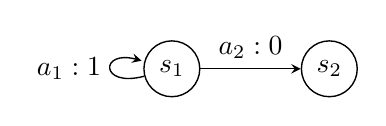
\begin{tikzpicture}[->,>=stealth, line width = 0.5 pt,node distance = 2 cm]

\node [circle, draw] (one) {$s_1$};
\node [circle, draw] (two) [right of=one] {$s_2$};
\path (one) edge [loop left] node  {$a_1:1$}(one);
\path (one) edge node [above, sloped] {$a_2:0$} (two);
\end{tikzpicture}
\end{figure}

\noindent Consider the following infinite-horizon MDP. The initial state is always $s_1$, and the episode terminates when $s_2$ is reached. The agent receives reward 1 for taking action $a_1$ and reward 0 for taking action $a_2$. In this case, we can define the policy with a single parameter $\theta$:
$$\pi_{\theta}(a_1|s_1) = \theta, \ \ \ \pi_{\theta}(a_2|s_1) = 1-\theta$$


\noindent{\bf (a)} 
Use policy gradients to compute the gradient of the expected return of $\pi_\theta$ with respect to the parameter $\theta$ (Eq. \ref{eq:4}). Do not use discounting.
\newline
You may find this fact useful:
$$\sum^{\infty}_{k=1}k\alpha^{k-1} = \frac{d}{d\alpha}\sum^{\infty}_{k=1}\alpha^{k} $$
\newline
\noindent{\bf (b)} Compute the expected return of the policy $\pi_\theta$ directly (Eq. \ref{eq:1}). Compute the gradient of this expression and verify that it matches your result in {\bf (a)}.
\newline

\noindent{\bf (c)} Reward-to-go can be helpful and improve the statistical qualities of our policy gradient. Apply reward-to-go as an advantage estimator. Write the new policy gradient (Eq. \ref{eq:5}), and verify that it is unbiased.

\newpage
\vskip \gap \noindent{\bf (2) Bounding Error in Approximate Policy Iteration  (10 points)}
\newline

\noindent In this problem, we look at how errors in approximating the value function affect the performance of a policy during policy iteration.
\newline

\noindent Let’s assume we are in an infinite horizon MDP with discount factor $\gamma$. We have a reference policy $\pi$ whose true value function is $V^\pi(s)$. We collect rollouts with $\pi$, and fit a neural network to approximate this value function, where $\hat V(s) \approx V^\pi(s)$. 
\newline

\noindent Let’s assume we did a really good job and can guarantee that the error from the fit is at most $\epsilon$. More formally, let $|| V^\pi - \hat V||_{\infty} \leq \epsilon$.\footnote{Note: $|| x ||_{\infty}$ is the L-infinity norm}
\newline

\noindent We now choose a greedy policy to improve upon policy $\hat{\pi}$:
$$\hat \pi(s) = \argmax_a \left[R(s,a) +  \gamma \sum_{s'} P(s'|s,a)\hat V(s')\right]$$
\noindent Note that this is exactly the policy improvement step, except the value function is substituted with our approximate value function. We want to know how the greedy policy  $\hat \pi(s)$ performs with respect to $\pi (s)$. 
\newline

\noindent Let $V^{\hat \pi}(s)$ be the value of the greedy policy $\hat \pi(s)$. Prove the following:

$$|V^{\pi}(s) -V^{\hat \pi}(s)| \leq  \frac{2\gamma \epsilon}{1-\gamma} \text{\;\;, for all $s$}$$

\noindent In other words, $\hat{\pi}$ can end up doing much worse than $\pi$. Additionally, even though the error from fitting the value was $\epsilon$, the performance error scales up by a factor of $\frac{1}{1-\gamma}$. 
\newline
\newline

\noindent \textit{Hint}:
One way to approach the question would be:
\begin{enumerate}
    \item For any policy we have,
$$V^{\pi}(s) = R(s,\pi(s)) + \gamma \sum_{s'} P(s'|s,\pi(s)) V^{\pi}(s')$$ 
Use this substitution to expand $V^{\pi}(s) -V^{\hat \pi}(s)$.
\item Next, note that you need to establish a relationship between $\pi(s)$ and $\hat \pi(s)$. Exploit the following observation: $\hat \pi(s) = \argmax_a f(s,a) $ must imply $f(s,\hat \pi(s))  \geq f(s,\pi(s))$ for any policy $\pi$.
\item Use these facts to obtain the following intermediate result. For any $s$,
$$V^{\pi}(s) -V^{\hat \pi}(s) \leq 2\gamma \epsilon + \gamma\sum_{s' \in \mathcal S} \Pr[s' | s, \hat \pi(s)](V^\pi(s') - V^{\hat \pi}(s'))$$
From the above, you should be able to prove the final result for all $s$.
\end{enumerate}

\newpage
\vskip \gap \noindent{\bf (3) Extra Credit (Mandatory for 5756): Reward Shaping with an Approximate Value Function (5 points)} 
\newline

\noindent Previously, we saw how acting greedily with an approximate value function can result in a \emph{worse} policy. Instead, what if we use the approximate value function to \emph{shape the reward}? 
\newline
 
\noindent Let's define a \emph{reward bonus} using the approximate value function from Q2. 

$$F(s,s') = \gamma \hat V(s') - \hat V(s)$$

\noindent This extra reward is gained whenever we transition from state $s$ to state $s'$. 
Informally, we are giving a small intermediate reward for moving toward states of higher value. Adding these intermediate rewards helps in speeding up a policy's convergence in environments with sparse rewards.

\noindent At each step $i$ of an episode, the shaped reward $R_i$ is then defined as
$$R_i = r_i + F(s_i,s_{i+1})$$
where $r_i$ is the base reward $r(s_i, a_i)$ received for step $i$. We continue to use a \emph{discount factor} of $\gamma$ in computing total reward.
\newline

\noindent{\bf (a)} \noindent Consider a given episode of potentially infinite-length, of visited states $s_0, s_1,...$ 

\noindent Write out the total reward received in the shaped environment, expressed in terms of the total reward that would have been accrued in the unshaped environment. What is noticeable about this relationship? 
\newline

\noindent{\bf (b)} Show that the performance of the optimal policy $\hat \pi$ computed with the shaped rewards is the same as the performance of the optimal policy $\pi^*$ without reward shaping. Formally, prove that:
$$||V^{\pi^*} -V^{\hat \pi}||_{\infty} = 0 $$

\end{document}
